In the model proposed in this work, the weight of the disk galaxy is supported by the turbulenc einjected by supernoave.
This links density and star formation together; a higher density leads to a feedback effect which leads to more star formation and hence a higher supernovae rate.
In equilibrium, these two are in balance, and there can be a relation formed between the surface star formation rate and surface gas density.

Once this star formation relation (which is similar to the Kennicut-Schmidt law described above) has been formulated, it can be combined with calibration simulations provided by \citet{martizzi2015} that give the relation between dispersion injected from supernovae and surface gas density.

\begin{figure}
    \centering
    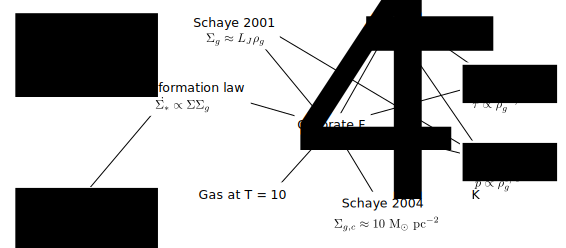
\includegraphics[width=\textwidth]{flowchart.pdf}
    \caption{This flowchart shows the overall process of building the model.
    It may be helpful to the reader when attempting to follow the construction; there are a number of elements required at any given time.}
    \label{fig:flowchart}
\end{figure}
